\documentclass[a4paper, parskip=half, DIV15]{scrartcl}
\usepackage[T1]{fontenc}
\usepackage[latin1]{inputenc}
\usepackage[ngerman]{babel}
%-------------- Kopf- und Fusszeile
\newcommand{\authorinfo}{Andreas Linggi, Stefan Steiner}
% �usserer Kopf
		\newcommand{\oheaderinfo}{Mathematisches Seminar}
% innerer Kopf
		\newcommand{\iheaderinfo}{}
% zentrierter Kopf
		\newcommand{\cheaderinfo}{}
%------- Rand falls eingeschaltet
%\newcommand{\randabstand}{1.5cm}
%--------------------------------------------- Schriften
%------- Schriften Kopf- und Fusszeile
\newcommand{\headfootnotefont}{\scriptsize\upshape}
%------- Schrift von Listenelementen
\newcommand{\listfont}{\sffamily}
%--------------------------------------------- Name von Eigener Liste
\newcommand{\nameoflist}{\oheaderinfo \hspace{1cm}\small{\authorinfo} \hspace{3cm}\today}

%\usepackage[style=ieee,backend=bibtex]{biblatex}
\usepackage[style = ieee,backend=bibtex]{biblatex}
\bibliography{quellen}

\usepackage[ngerman]{varioref}
\usepackage[german]{fancyref}
\usepackage{graphicx,amssymb,amsmath,relsize}
%--------------------------------------------- Kopf- und Fusszeile
\usepackage{scrpage2}
\pagestyle{scrheadings}
\clearscrheadings
\clearscrplain
\ifoot{\headfootnotefont\authorinfo}
%------ % SeitenZahlen outer foot
\usepackage{lastpage}
\ofoot{\headfootnotefont Seite \thepage { }von \pageref{LastPage}}
%------
\ohead{\headfootnotefont\oheaderinfo}
\ihead{\headfootnotefont\iheaderinfo}
\chead{\headfootnotefont\cheaderinfo}
\setheadsepline{.4pt} 											% Linie unter der Kopfzeile
%--------------------------------------------- TikZ und GNU Plot
\usepackage{tikz}
%---------------------------------------------
\usepackage{hyperref}
%--------------------------------------------- Tabellen
\usepackage{array}
\usepackage{booktabs}
\usepackage{multirow}
\usepackage{multicol}
\newcommand{\tabH}[1]{\parbox[1pt][#1em][c]{0cm}{}}
\newcommand{\red}[1]{\textcolor{red}{#1}}
\newcommand{\blue}[1]{\textcolor{blue}{#1}}
\newcommand{\orange}[1]{\textcolor{orange}{#1}}

%------------------- C-Code ------------------- %
\definecolor{colorkeywordstyle}{RGB}{127,0,127}
\definecolor{colorcommentstyle}{RGB}{0,116,0}
\definecolor{colorstringstyle}{RGB}{196,26,22}
\definecolor{colorbackground}{RGB}{240,240,240}
\definecolor{royalblue}{rgb}{0.15,0.25,0.55}
\definecolor{black}{rgb}{0,0,0}

\usepackage{listings}
\lstnewenvironment{code}[1][]
  {\lstset{
  	backgroundcolor =		\color{colorbackground},
    language =				C++,			
    basicstyle =    		\ttfamily,
    breaklines = 			true,
    frame = 				none,
    columns =				flexible,
    keepspaces = 			true,
    keywordstyle=			\color{colorkeywordstyle},
    identifierstyle	=\color{royalblue},
    showstringspaces =		false,
    extendedchars =			true,   
    commentstyle = 			\color{colorcommentstyle},,
    numbers = 				left,
    numbersep = 			2pt,
    numberstyle =			\tiny,
    rulecolor=\color{black}, 
    stepnumber =			1,
    tabsize = 				4,
  }}{\vspace{0em}}
\lstset{
  	backgroundcolor =		\color{colorbackground},
    language =				C++,			
    basicstyle =    		\ttfamily,
    breaklines = 			true,
    frame = 				none,
    columns =				flexible,
    keepspaces = 			true,
    keywordstyle=			\color{colorkeywordstyle},
    identifierstyle	=\color{royalblue},
    showstringspaces =		false,
    extendedchars =			true,   
    commentstyle = 			\color{colorcommentstyle},,
    numbers = 				left,
    numbersep = 			2pt,
    numberstyle =			\tiny,
    rulecolor=\color{black}, 
    stepnumber =			1,
    tabsize = 				4,
}
%---------------------------------------------
\newcommand{\dunderline}[1]{\underline{\underline{#1}}}



\begin{document}

\tableofcontents

\section{Aufgabenstellung}
Um ein Problem der Mathematik besser zu verstehen, ist es oft sehr hilfreich, wenn dieses verst�ndlich beschrieben ist. Eine Visualisierung in Form eines Bildes oder kurzen Films ist dabei eine M�glichkeit dies zu bewerkstelligen.

Die Hauptaufgabe dieses Projektes, war es nun, die Greensche Funktion in zwei Dimensionen zu visualisieren. Die L�sung f�r eine Dimension wurde bereits in einem kurzen Film veranschaulicht \footnote{\url{https://www.youtube.com/watch?v=Wpi7Gf7V2HY}}. Es soll dabei zuerst eine partielle Differentialgleichung mithilfe des Greenschen Ansatzes gel�st und danach das visualisieren umgesetzt werden. Die Greensche Funktion erm�glicht die Berechnung eines Problems durch Supperposition. Darum sollten auch verschiedene Anfangswerte untersucht werden und wie diese sich auf die L�sungen auswirken. 

Als Differentialgleichung sei dabei ein Potentialproblem vorgegeben. Vorliegend ist eine leitende Platte, die am Rande geerdet sei. Wenn nun ein Potential an einem oder mehreren Punkten auf dieser Platte anliegt, ist es von Interesse zu wissen, welches Potential man nun an einem beliebigen Punkt auf der Platte misst. Die folgende partielle Differentialgleichung l�st dabei dieses Problem.
\begin{equation}
	\dfrac{\partial^2 u}{\partial x^2}+\dfrac{\partial^2 u}{\partial y^2} = f(x,y).
\end{equation}
Dabei sei hier noch auf die Arbeit von Reto Christen und Philip Solenthaler verwiesen. Diese haben das Potentialproblem genauer untersucht. 

\section{George Green}
Der Namensgeber f�r die Greensche Funktion ist George Green. Er war ein britischer Physiker und Mathematiker. Geboren wurde er 1793 in der N�he von Nottingham. Sein Vater betrieb eine M�hle und George Green arbeitete ebenfalls als M�ller. Nach dem Tod seines Vaters f�hrte er den M�hlenbetrieb fort. Bemerkenswert ist, dass Green nur etwa zwei Jahre in die Schule ging. Mathematische und Physikalische Grundlagen brachte er sich selber bei. Der Ort an dem er lernte war seine M�hle. Da nie ein Portrait von ihm angefertigt wurde, gibt es kein Bild von ihm. Darum wird anstatt seinem Konterfei jeweils eine Windm�hle verwendet um ihn darzustellen. Die Windm�hle gibt es �brigens immer noch. Green ver�ffentliche mit etwa dreissig Jahren seine erste Arbeit. Diese wurde kaum beachtet, ausser von einem adligen Mathematik namens Sir Edward Bromhead. Er ermutigte Green, im Alter von vierzig Jahren in Cambridge zu studieren. Interessant zu wissen ist dazu, dass dort zu dieser Zeit die Theorien von Laplace und Fourier noch nicht gelehrt wurden. Green hatte sich jedoch durch diese Theorie gelesen und sogar noch einige Erweiterungen hinzugef�gt. Vier Jahre nachdem er graduierte und kurz vor seinem internationalen Durchbruch stand, starb er 1841 jedoch an einer schweren Grippe. Dadurch geriet seine Arbeit f�r einige Zeit in Vergessenheit.

George Green ist besonders bekannt f�r das Greensche Theorem und die Greensche Funktion. Er besch�ftigte sich mit der L�sung von partiellen Differentialgleichungen und stellte damit unter anderem mathematische Hilfsmittel bereit, die sogar in der Quantenfeldtheorie im 20. Jahrhundert von Bedeutung waren.\cite{wiki:green}

Neben vielen anderen Pers�nlichkeiten wie Maxwell, Dirac oder Newton ist er in der Westminster Abbey in London mit einer Gedenktafel verewigt\cite{wiki:westminster}. Der Grund, warum George Green nicht so popul�r ist wie Gauss oder Maxwell, liegt wahrscheinlich darin, dass von seiner Zeit, als er in seiner M�hle gearbeitet hat, wenig  bekannt ist. Auch war er nur f�r sehr kurze Zeit in Cambridge t�tig. Trotzdem war es an dieser Stelle das Ziel, einen so einzigartigen Wissenschaftler, mehr als nur kurz zu erw�hnen.

	\begin{figure}[htb]                     \centering 
	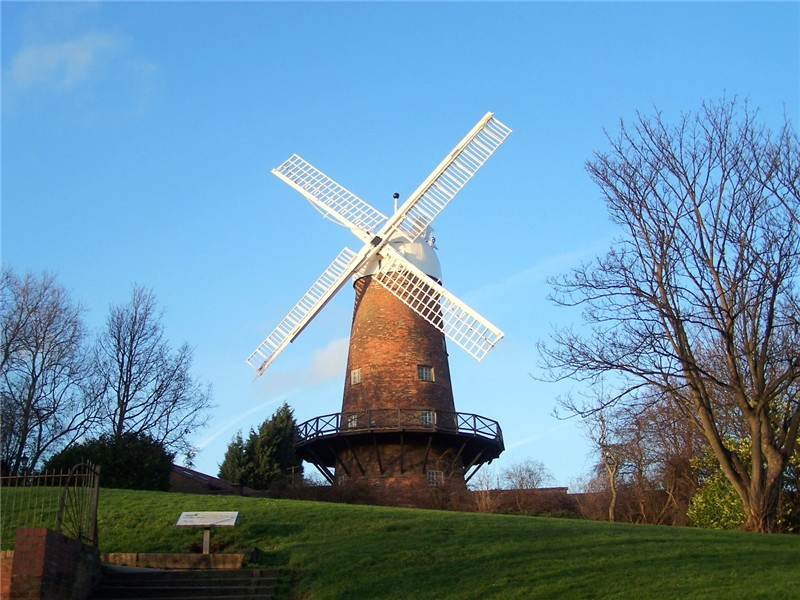
\includegraphics[width=8cm]{images/greens_windmill} 
	\caption{Windm�hle, in der Green f�r lange Zeit gearbeitet hat} 
	\label{fig:abb1} 
	\end{figure} 


\section{Algorithmus}
\begin{frame}
\frametitle{Algorithmus}

\[
	A=\left(
	\begin{array}{ccccc|ccccc|c|ccccc}
	    -4&     1&     0&\cdots&     0 &     1&     0&     0&\cdots&     0 &\cdots &      &      &      &      &      \\
	     1&    -4&     1&\cdots&     0 &     0&     1&     0&\cdots&     0 &\cdots &      &      &      &      &      \\
	     0&     1&    -4&\cdots&     0 &     0&     0&     1&\cdots&     0 &\cdots &      &      &     0&      &      \\
	\vdots&\vdots&\vdots&\ddots&\vdots &\vdots&\vdots&\vdots&\ddots&\vdots &       &      &      &      &      &      \\
	     0&     0&     0&\cdots&    -4 &     0&     0&     0&\dots &     1 &\cdots &      &      &      &      &      \\
	\hline
	     1&     0&     0&\cdots&     0 &    -4&     1&     0&\dots &     0 &\cdots &      &      &      &      &      \\
	     0&     1&     0&\cdots&     0 &     1&    -4&     1&\dots &     0 &\cdots &      &      &      &      &      \\
	     0&     0&     1&\cdots&     0 &     0&     1&    -4&\dots &     0 &\cdots &      &      &     0&      &      \\
	\vdots&\vdots&\vdots&\ddots&\vdots &\vdots&\vdots&\vdots&\ddots&\vdots &       &      &      &      &      &      \\
	     0&     0&     0&\cdots&     1 &     0&     0&     0&\cdots&    -4 &\cdots &      &      &      &      &      \\
	\hline
	\vdots&\vdots&\vdots&      &\vdots &\vdots&\vdots&\vdots&      &\vdots &\ddots &\vdots&\vdots&\vdots&      &\vdots\\
	\hline
	      &      &      &      &       &      &      &      &      &       &\cdots &    -4&     1&     0&\cdots&     0\\
	      &      &      &      &       &      &      &      &      &       &\cdots &     1&    -4&     1&\cdots&     0\\
	      &      &     0&      &       &      &      &     0&      &       &\cdots &     0&     1&    -4&\cdots&     0\\
	      &      &      &      &       &      &      &      &      &       &       &\vdots&\vdots&\vdots&\ddots&\vdots\\
	      &      &      &      &       &      &      &      &      &       &\cdots &     0&     0&     0&\cdots&    -4\\
	\end{array}
	\right) 
	\]

\end{frame}
\section{Visualisierung}
	
	Wir speichern die erhaltene Matrix in einem .csv File mit einer Genauigkeit von vier Nachkommastellen ab, was f�r eine Visualisierung absolut hinreichen ist. Anfangs benutzten wir MATLAB um aus dem CSV-File eine anst�ndige Visualisierung zu erhalten. Der Aufwand war gering und die Resultate waren schnell kontrollierbar.
	
	\lstinputlisting{./csvToMatrixAndPlot.m}
	
	Um das zu automatisieren benutzen wir sp�ter Gnuplot, welches sich mit C-Code ohne Probleme ansprechen l�sst und uns die Bilder automatisch mit dem vorgegebenen Einstellungen erstellt.
	
	Gnuplot ist ein Kommandozeilen basiertes OpenSource Tool, das aber auch mit GUI erh�ltlich ist. �ber eine Pipe lassen sich lassen sich alle Einstellungen vornehmen und aus dem .CSV-File ein PNG generieren.
	
	\lstinputlisting{./gnuplot.c}
	
	Mit der Green-Funtion k�nnen bei einer partiellen DGL 2. Ordnung einzelne Punkte berechnet werden. Um das zu visualisieren, berechnen wir einzelne Ringe bzw. Quadrate vom Zentrum ausgehen nach aussen. Man k�nnte nat�rlich auch jeder Punkt einzeln dazu nehmen, was mehr Berechnungen erfordert.
	
		\[
			f=\left(
			\begin{array}{ccccc}
			    f_{11}& f_{12}& f_{13}& f_{14}& f_{15}\\
				f_{21}& f_{22}& f_{23}& f_{24}& f_{25}\\
				f_{31}& f_{32}& \red{f_{33}}& f_{34}& f_{35}\\
				f_{41}& f_{42}& f_{43}& f_{44}& f_{45}\\
				f_{51}& f_{52}& f_{53}& f_{54}& f_{55}\\
			\end{array}
			\right) \Rightarrow
			\left(
			\begin{array}{ccccc}
			    f_{11}& f_{12}& f_{13}& f_{14}& f_{15}\\
				f_{21}& \red{f_{22}}& \red{f_{23}}& \red{f_{24}}& f_{25}\\
				f_{31}& \red{f_{32}}& \red{f_{33}}& \red{f_{34}}& f_{35}\\
				f_{41}& \red{f_{42}}& \red{f_{43}}& \red{f_{44}}& f_{45}\\
				f_{51}& f_{52}& f_{53}& f_{54}& f_{55}\\
			\end{array}\right)
			\Rightarrow
			\left(\red{
			\begin{array}{ccccc}
			    f_{11}& f_{12}& f_{13}& f_{14}& f_{15}\\
				f_{21}& f_{22}& f_{23}& f_{24}& f_{25}\\
				f_{31}& f_{32}& f_{33}& f_{34}& f_{35}\\
				f_{41}& f_{42}& f_{43}& f_{44}& f_{45}\\
				f_{51}& f_{52}& f_{53}& f_{54}& f_{55}\\
			\end{array}}
			\right)
			\]

	
	Diese einzelnen Schritte werden vollst�ndig berechnet und dann als .csv abgespeichert. Die Bilder werden nachdem alle Einzelschritte berechnet wurden aus den Dateien wiederum parallelisiert in einer \verb|for|-Schleife zu .png Bilddateien verarbeitet. Die Skalierung der z-Achse wird direkt aus den Daten des letzten Schrittes berechnet, was uns eine optimale Darstellung garantiert. Aus den Bilddateien wird am Schluss optional noch ein Video erstellt.
		
\section{FITS Dateiformat}\label{sec:FITS}

Flexible Image Transport System ist die ausgeschriebene Bezeichnung f�r das Wort FITS. Es ist ein quelloffenes Dateiformat, womit Daten verlustlos abgespeichert werden k�nnen. Die Nasa entwickelte es und in der Astronomie hat es sich als Standardformat etabliert.  Informationen k�nnen in verschiedenen Layern abgelegt werden. Das bedeutet, ein Gitterpunkt in einem Datenfeld kann unterschiedliche Informationen enthalten. Angenehm ist ausserdem, dass die Werte direkt in Flisskommadarstellung abgespeichert werden k�nnen.\cite{nasa:fits}

Wir haben es in diesem Projekt als Eingabebild verwendet, weil wir mit einem einfachen Bildbearbeitungsprogramm Testbilder herstellen konnten.  


\printbibliography
\listoffigures

\end{document}